
%%% use twocolumn and 10pt options with the asme2ej format
\documentclass[twocolumn,10pt]{asme2ej}

\usepackage{epsfig} %% for loading postscript figures
\usepackage{listings}
\usepackage{amsmath}
\usepackage{graphicx}
\usepackage{grffile}
\usepackage{pdfpages}
\usepackage{algpseudocode}
\usepackage{courier}
\usepackage{tikz}
\newcommand*\circled[1]{\tikz[baseline=(char.base)]{
            \node[shape=circle,draw,inner sep=2pt] (char) {#1};}}
%\usepackage{multicol}


% Custom colors
\usepackage{color}
\usepackage{listings}
\usepackage{framed}
\usepackage{caption}
\usepackage{bm}
\captionsetup[lstlisting]{font={small,tt}}

\definecolor{mygreen}{rgb}{0,0.6,0}
\definecolor{mygray}{rgb}{0.5,0.5,0.5}
\definecolor{mymauve}{rgb}{0.58,0,0.82}

\lstset{ %
  backgroundcolor=\color{white},   % choose the background color; you must add \usepackage{color} or \usepackage{xcolor}
  basicstyle=\ttfamily\footnotesize, % the size of the fonts that are used for the code
  breakatwhitespace=false,         % sets if automatic breaks should only happen at whitespace
  % breaklines=true,                 % sets automatic line breaking
  captionpos=b,                    % sets the caption-position to bottom
  commentstyle=\color{mygreen},    % comment style
  deletekeywords={...},            % if you want to delete keywords from the given language
  escapeinside={\%*}{*)},          % if you want to add LaTeX within your code
  extendedchars=true,              % lets you use non-ASCII characters; for 8-bits encodings only, does not work with UTF-8
  frame=single,                    % adds a frame around the code
  keepspaces=true,                 % keeps spaces in text, useful for keeping indentation of code (possibly needs columns=flexible)
  columns=flexible,
  keywordstyle=\color{blue},       % keyword style
  language=Python,                 % the language of the code
  morekeywords={*,...},            % if you want to add more keywords to the set
  numbers=left,                    % where to put the line-numbers; possible values are (none, left, right)
  numbersep=5pt,                   % how far the line-numbers are from the code
  numberstyle=\tiny\color{mygray}, % the style that is used for the line-numbers
  rulecolor=\color{black},         % if not set, the frame-color may be changed on line-breaks within not-black text (e.g. comments (green here))
  showspaces=false,                % show spaces everywhere adding particular underscores; it overrides 'showstringspaces'
  showstringspaces=false,          % underline spaces within strings only
  showtabs=false,                  % show tabs within strings adding particular underscores
  stepnumber=1,                    % the step between two line-numbers. If it's 1, each line will be numbered
  stringstyle=\color{mymauve},     % string literal style
  tabsize=4,                       % sets default tabsize to 2 spaces
}



%% The class has several options
%  onecolumn/twocolumn - format for one or two columns per page
%  10pt/11pt/12pt - use 10, 11, or 12 point font
%  oneside/twoside - format for oneside/twosided printing
%  final/draft - format for final/draft copy
%  cleanfoot - take out copyright info in footer leave page number
%  cleanhead - take out the conference banner on the title page
%  titlepage/notitlepage - put in titlepage or leave out titlepage
%
%% The default is oneside, onecolumn, 10pt, final

\title{MAE 267 -- Project 4\\Parallel, Multi-Block, Finite-Volume Methods\\For Solving 2D Heat Conduction}

%%% first author
\author{Logan Halstrom
    \affiliation{
	PhD Graduate Student Researcher\\
	Center for Human/Robot/Vehicle Integration and Performance\\
	Department of Mechanical and Aerospace Engineering\\
	University of California, Davis\\
	Davis, California 95616\\
    Email: ldhalstrom@ucdavis.edu
    }
}

\begin{document}
\maketitle

%%%%%%%%%%%%%%%%%%%%%%%%%%%%%%%%%%%%%%%%%%%%%%%%%%%%%%%%%%%%%%%%%%%%%%
\section{Statement of Problem}

This analysis demonstrates the fundamentals of parallel computing through the numerical solution of the steady-state, two-dimensional temperature distribution of a 1m x 1m steel block with properties listed in Table~\ref{props}.

%STEEL PROPERTIES TABLE
\vspace{-1.8em}
\begin{table}[htb]
\begin{center}
\caption{Steel Block Properties}
\begin{tabular}{|l | c|}
\hline
Dimensions & 1m x 1m \\
\hline
Thermal Conductivity & $k=18.8\frac{W}{m \cdot K}$  \\
\hline
Density & $\rho=8000\frac{kg}{m^3}$  \\
\hline
Specific Heat Ratio & $c_p=500$  \\
\hline
\end{tabular}
\label{props}
\end{center}
\end{table}
\vspace{-2.3em}

The demonstration of parallel computing techniques was accomplished in stages, starting with a serial (single-processor) solution of a single grid of dimensions 101x101 and 501x501, which serves as a solver basis and performance benchmark for later parallel codes.

The next stage was to divide the grid into NxM subdomains (blocks), on each of which the solution for a given iteration was calculated independently.  5x4 and 10x10 block decompositions of both previous grid dimensions were solved to demonstrate compartmentalization of solver processes, which is a necessary step for distributing processes in parallel computing.

Finally, the code will be adapted to solve multi-block decompositions on multiple processors for the 501x501 grid decomposed into 10x10 blocks running on 4 to 8 processors.  This stage steps closer to that solution by performing domain decomposition and processor distribution for 5x4 and 10x10 blocks on 4 and 6 processors, and saving the decompositions to restart files to be loaded by the parallel solver.


%%%%%%%%%%%%%%%%%%%%%%%%%%%%%%%%%%%%%%%%%%%%%%%%%%%%%%%%%%%%%%%%%%%%%%%%
\section{Methods and Equations}

The core of this demonstration code is the heat transfer solver developed in the first project, but a number of domain decomposition functions have since been included, as will be detailed in this section.

\subsection{Grid Initialization}

The numerical solution is initialized with the Dirichlet boundary conditions (Eqn~\ref{dirichlet}) using a single processor.

\begin{equation}
\begin{split}
T_{BCs} = &\left\{ \begin{array}{lll}
    \mbox{$5.0 \left[ \sin\left( \pi x_p \right) + 1.0 \right]$} & \mbox{for } &j = j_{max} \\
    \mbox{$\left| \cos\left( \pi x_p \right)\right|+1.0$} & \mbox{for } &j = 0 \\
    \mbox{$3.0 y_p + 2.0$} & \mbox{for } &i = 0, \, i_{max}
     \end{array} \right.
\end{split}
\label{dirichlet}
\end{equation}

\begin{equation}
\begin{split}
   rot &= 30.0 \frac{\pi}{180.0} \\
   x_p(i) &= \cos \left[ 0.5\pi \frac{i_{max}-i}{i_{max}-1} \right] \\
   y_p(j) &= \cos \left[ 0.5\pi \frac{j_{max}-j}{j_{max}-1} \right] \\
   x &= x_p \cos(rot) + (1.0 - y_p) \sin(rot) \\
   y &= y_p \cos(rot) + x_p \sin(rot)
\end{split}
\label{grideqn}
\end{equation}

\noindent Square grids are generated according to Eqn~\ref{grideqn} to create non-uniform spacing in both the x and y directions (with finer spacing at the larger indices).  The ``prime'' system is then rotated by angle $rot$ to create the final grid.

\subsection{Numerical Solver}

The solver developed for this analysis utilizes a finite-volume numerical solution method to solve the transient heat conduction equation (Eqn~\ref{heat}).

\begin{equation}
\begin{split}
\rho c_p \frac{\partial T}{\partial t} =
    k \left[ \frac{\partial^2 T}{\partial x^2}
    + \frac{\partial^2 T}{\partial y^2} \right]
\end{split}
\label{heat}
\end{equation}

\noindent To solve Eqn~\ref{heat} numerically, the equation is discretized according to a node-centered, finite-volume scheme, where first-derivatives at the nodes are found using Green's theorem integrating around the secondary control volumes.  Trapezoidal, counter-clockwise integration for the first-derivative in the x-direction is achieved with Eqn~\ref{FVx1st}.

\begin{equation}
\begin{split}
\frac{\partial T}{\partial x} = \frac{1}{2Vol_{i+\frac{1}{2},j+\frac{1}{2}}}
    \left[ \left(T_{i+1,j} + T_{i+1,j+1} \right)Ayi_{i+1,j} \right. \\
    \left. - \left(T_{i,j} + T_{i,j+1} \right)Ayi_{i,j} \right. \\
    \left. - \left(T_{i,j+1} + T_{i+1,j+1} \right)Ayi_{i,j+1} \right. \\
    \left. - \left(T_{i,j} + T_{i+1,j} \right)Ayi_{i,j} \right]
\end{split}
\label{FVx1st}
\end{equation}

\noindent A similar scheme is used to find the first-derivative in the y-direction.


\subsection{Subdomain Decomposition}

After grid initialization, the grid is divided into N blocks in the x/I direction and M blocks in the y/J direction, creating a total number of blocks $NBLK=N\cdot M$.  All blocks are constrained to have the same number of nodes, so the dimensions of every block $IBLKMAX$ and $JBLKMAX$ are calculated in Eqn~\ref{iblocksize} as a fraction of the total number of nodes in each direction, including one point overlap at each inter-block boundary (Ghost nodes are excluded for the moment).  In the I-direction, the total number of nodes including overlap (Eqn~\ref{idirpoints}) is:

\vspace{-1em}
\begin{equation}
\begin{split}
IMAX_{tot} = IMAX + (N-1)
\end{split}
\label{idirpoints}
\end{equation}
\vspace{-1em}

\noindent and the total number of nodes per block in the I-direction (Eqn~\ref{iblocksize}) is:

\vspace{-1em}
\begin{equation}
\begin{split}
IMAXBLK = \frac{IMAX_{tot}}{N} = \frac{IMAX + (N-1)}{N} = 1 + \frac{IMAX-1}{N}
\end{split}
\label{iblocksize}
\end{equation}

\noindent Note: For points in J-direction, replace I with J and N with M

Blocks are distributed from 1 to NBLK starting in the lower-left corner of the grid and zipping left to right (the x/I/N direction), then up one (the y/J/M direction) starting again at the left.  This is accomplished by two DO loops, the outer loop stepping through J from 1 to M and the inner loop stepping through I from 1 to N. Block locations are stored by assigning global starting indices to each block according to Eqn~\ref{blockstartingindex}.

\begin{equation}
\begin{split}
IMIN_{block} = IMIN_{global} + (IMAXBLK-1)(I-1)
\end{split}
\label{blockstartingindex}
\end{equation}

\noindent where I counts blocks in the direction of N and $IMIN_{global}=1$.  The first block in the N-direction has a global starting index of 0, and IMAXBLK must be reduced by one to account for the single-point overlap at block boundaries.

Information for each block is stored as an element in an array of BLKTYPE derived data types.  BLKTYPE stores local mesh, temperature, and solver information as well as the block ID, global  indices, iteration bounds to prevent overwriting boundary conditions (discussed in Section~\ref{neighborsec}), and neighbor identification information.

\subsection{Processor Distribution}

For the parallel code, blocks are distributed among $NPROCS$ processors (determined in `miprun’ call), with the goal of equal load balancing for all processors (Eqn~\ref{loadbalance}).  Load balance is the ratio of a processor's workload to the ``Perfect Load Balance'' ($PLB$), the total load of all blocks divided by $NPROCS$.  In this code, a block's load is refered to as its $SIZE$, so a processor's work load is equal to the sum of the $SIZEs$ of its blocks.

\vspace{-1em}
\begin{equation}
\begin{split}
P_{LoadBalance} = \frac{SUM(SIZEs)}{PLB}
\end{split}
\label{loadbalance}
\end{equation}

The workload of each block ($SIZE$) is calculated as a weighted sum (Eqn~\ref{blockload}) of its geometric cost $GEOM$ due to grid size (Eqn~\ref{geomcost}) and communication cost $COMM$ due to boundary size (~\ref{commcost}).  Geometric cost is essentially the node area of the block iteration bounds:

\vspace{-1em}
\begin{equation}
\begin{split}
GEOM = (IMAXLOC - IMINLOC) \cdot (JMAXLOC - JMINLOC)
\end{split}
\label{geomcost}
\end{equation}

\noindent Geometric cost will be greater for cells that are not on physical boundaries as they require more ghosts nodes for their inter-block boundaries.  Communication cost is calculated as the total length of all faces and corners at interblock boundaries:

\vspace{-1em}
\begin{equation}
\begin{split}
&COMM(i) =
      \begin{cases}
        0, & \text{if BC} \\
        IMAXBLK - IMINBLK, & \text{if N or S Face Neighbor} \\
        JMAXBLK - JMINBLK, & \text{if E or W Face Neighbor} \\
        1, & \text{if Corner Neighbor}
      \end{cases} \\
&COMM = SUM(COMM(i))
\end{split}
\label{commcost}
\end{equation}
\noindent where Eqn~\ref{commcost} must be evaluated for all faces and corners of a given block and the results must be summed.

Weights of each type of cost are currently set to make the maximum possible geometric cost equal to the maximum possible communication cost, as accomplished by Eqn~\ref{blockload}.

\vspace{-1em}
\begin{equation}
\begin{split}
&WGEOM = 1 \\
&WCOMM = FACTOR \cdot \frac{(IMAXBLK+2)(JMAXBLK+2)}{(2 \cdot IMAXBLK)+(2 \cdot IMAXBLK)+4 } \\
&SIZE = (WGEOM \cdot GEOM) + (WCOMM \cdot COMM)
\end{split}
\label{blockload}
\end{equation}
\noindent where $FACTOR$ is a number that can be varied to tune cost weighting, but is currently set to 1.

Once block loads are calculated, they are sorted by size in order of greatest to least.  They are then distributed to the processors in this order, where each block is assigned to the current processor with the least load.  This produces the theoretical load balancing presented in Section~\ref{results}.  Actual load balancing performance will be determined in Project 5 and tuning will be performed to optimized load balancing.

\subsection{Ghost Nodes and Neighbor Indentification} \label{neighborsec}

In order for each block to function independently for a given iteration of the solver, it must know information about the nodes immediately outside of its boundaries, or, in other words, the interior nodes of its neighbors.  To preserve block independence, each block stores the information it needs from its neighbor at the beginning of each iteration in extra, off-block nodes called “ghost nodes”.  These nodes change the local size of each block and necessitate the local iteration parameters $ILOCMIN$, $ILOCMAX$, etc. discussed earlier.

To update each ghost boundary, the identity of the neighbor block for each face is stored in a variable $NB$, which is a neighbor derived data type $NBRTYPE$, which contains IDs for the north, south, east, and west faces and the north east, south east, south west, and north west corners.  If the block boundary is a physical boundary instead of an inter-block boundary, the corresponding neighbor identifier is instead set to 0 to indicate a BC boundary.  For parallel computing, if a neighbor block is on a different processor (indicating a processor boundary), the neighbor block ID is negated to indicate as such while still preserving the neighbor block ID.

Neighbor information is used to populate a linked list for each boundary type with block IDs so that all similar types of boundaries may be looped through in sequence, rather than using logical sorting at the beginning of each iteration.  (Linked lists were shown to produces a 25\% speed-up compared to logical sorting for the serial, multi-block code).

When moving to parallel computing, the ID of the neighbor block’s processor must also be bookeeped, as it is required information for accessing the neighbor block for ghost updating.  In addition to the neighbor block’s processor, the local index of the neighbor block on it’s processor must also be stored for this same reason.  Thus, this data is stored in corresponding $NBRTYPEs$.  Neighbor processor ID’s are stored in the variable $NP$.  If a block boundary is a BC, the processor ID is negated to indicate as such.  Local indices of neighbor blocks on neighbor processors are stored in $NBLOC$ and are set to 0 if a boundary is a BC.

\subsection{Configuration Restart Files}
After all of the above mentioned initialization processes have been completed, this information is stored in restart files so that the solver may start up independently from these files without needing to determine boundary procedures.  Neighbor information, grid, and temperature files are written for each processor.

%%%%%%%%%%%%%%%%%%%%%%%%%%%%%%%%%%%%%%%%%%%%%%%%%%%%%%%%%%%%%%%%%%%%%%

% %%\vspace{-2em}
% \begin{figure}[htb]
% \begin{center}
% \includegraphics[width=0.5\textwidth]{../Results/finalMulti/501_10x10.png}
% \caption{Steady-state temperature solution for 501x501 grid decomposed into 10x10 blocks}
% \label{501x10x10}
% \end{center}
% \end{figure}
% %%\vspace{-2em}

% %%\vspace{-2em}
% \begin{figure}[htb]
% \begin{center}
% 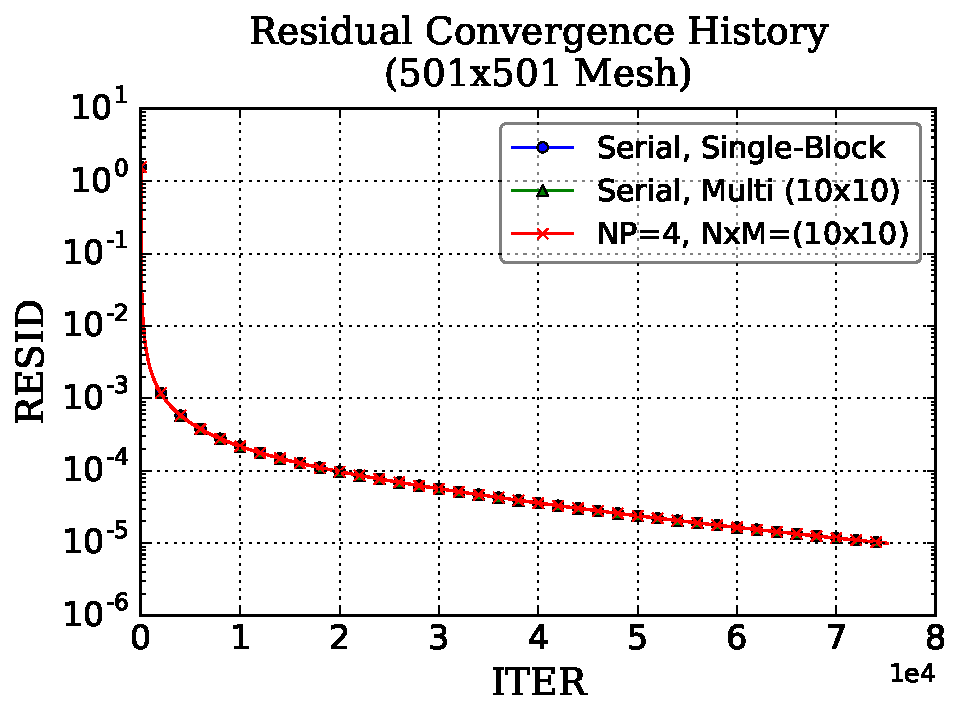
\includegraphics[width=0.5\textwidth]{../Results/ResHist.png}
% \caption{Residual history for solving a 501x501 grid with a single block solver and a 10x10 multi-block solver}
% \label{reshist}
% \end{center}
% \end{figure}
% %%\vspace{-2em}

\section{Results and Discussion} \label{results}



%LOAD BALANCING
\vspace{-1.8em}
\begin{table}[htb]
\begin{center}
\caption{Processor Theoretical Load Balances}
\begin{tabular}{|c | c c c c|}
\hline
\textbf{$NPROCS$} & 4   & 4   & 6     & 6     \\
\textbf{$MxN$}    & 5x4 & 10x10 & 5x4 & 10x10 \\
\hline
\textbf{Proc0}    & load & load & load & load \\
\textbf{Proc1}    & load & load & load & load \\
\textbf{Proc2}    & load & load & load & load \\
\textbf{Proc3}    & load & load & load & load \\
\textbf{Proc4}    & N/A & N/A & load & load \\
\textbf{Proc5}    & N/A & N/A & load & load \\

\hline
\end{tabular}
\label{lbtable}
\end{center}
\end{table}
\vspace{-2.3em}



%%%%%%%%%%%%%%%%%%%%%%%%%%%%%%%%%%%%%%%%%%%%%%%%%%%%%%%%%%%%%%%%%%%%%%%%
\section{Conclusion}

Decomposing the domain introduced unforseen complications in adapting the single block solver.  In some cases, it was as simple as adding a third loop for the block number, but in others (especially in updating the ghost nodes) considerable thought and error-checking was required.  This implies that adapting the code for parallel processing will be an equally complicated step, so it is beneficial that we are adapting our codes modularly in stages.

%%%%%%%%%%%%%%%%%%%%%%%%%%%%%%%%%%%%%%%%%%%%%%%%%%%%%%%%%%%%%%%%%%%%%%%%
% \section{References}
% \begin{description}
% \item[] 1. Bogard, D.G., Teiderman, W.G. ``Burst detection with single-point velocity measurements'', \emph{Journal of Fluid Mechanics}, 162:389-413, 1986.
% \end{description}








%%%%%%%%%%%%%%%%%%%%%%%%%%%%%%%%%%%%%%%%%%%%%%%%%%%%%%%%%%%%%%%
% \clearpage
\onecolumn
\appendix       %%% starting appendix

% \section*{Appendix A: Solver Performace Comparison} \label{times}
% \lstinputlisting[caption=Single block solver performance, language={}]{../Results/finalSingle/SolnInfo.dat}
% \lstinputlisting[caption=Multi block solver performance, language={}]{../Results/finalMulti/SolnInfo.dat}

% \section*{Appendix B: Multi-Block Grid Decomposition Code}
% \lstinputlisting[caption=Grids are decomposed into blocks and information pertaining to neighbors is stored using the GRIDMOD module, language=Fortran]{../modules.f90}

% \section*{Appendix C: Multi-Block Solver Subroutines}
% \lstinputlisting[caption=Main subroutines used for solving heat transfer on a multi-block grid, language=Fortran]{../subroutines.f90}

% \clearpage

% \section*{Appendix D: Multi-Block Plot3D Reader-Writer}
% \lstinputlisting[caption=Code for saving formatted multiblock PLOT3D solution files and reading restart files, language=Fortran]{../inout.f90}

% % \clearpage
% \section*{Appendix E: Other Relevant Codes}
% \lstinputlisting[caption=Wrapper program, language=Fortran]{../main.f90}



%%%%%%%%%%%%%%%%%%%%%%%%%%%%%%%%%%%%%%%%%%%%%%%%%%%%%%%%%%%%%%%%%%%%%%
%\clearpage


%%%%%%%%%%%%%%%%%%%%%%%%%%%%%%%%%%%%%%%%%%%%%%%%%%%%%%%%%%%%%%%%%%%%%%
% The bibliography is stored in an external database file
% in the BibTeX format (file_name.bib).  The bibliography is
% created by the following command and it will appear in this
% position in the document. You may, of course, create your
% own bibliography by using thebibliography environment as in
%
% \begin{thebibliography}{12}
% ...
% \bibitem{itemreference} D. E. Knudsen.
% {\em 1966 World Bnus Almanac.}
% {Permafrost Press, Novosibirsk.}
% ...
% \end{thebibliography}

% Here's where you specify the bibliography style file.
% The full file name for the bibliography style file
% used for an ASME paper is asmems4.bst.
%\bibliographystyle{asmems4}

% Here's where you specify the bibliography database file.
% The full file name of the bibliography database for this
% article is asme2e.bib. The name for your database is up
% to you.
%\bibliography{asme2e}

%%%%%%%%%%%%%%%%%%%%%%%%%%%%%%%%%%%%%%%%%%%%%%%%%%%%%%%%%%%%%%%%%%%%%%


\end{document}
